\section{L'architecture mise en place}
\label{sec:architecture}

\paragraph{}
La création d'un site web est une tâche complexe et il convient de mettre en place des outils robustes et éprouvés plutôt que de tout créer de zéro.
Il est aussi primordial de structurer les différents composants de l'application de manière intelligente de manière à obtenir un tout cohérent, maintenable et extensible.
Sachant que Altissia gère une quarantaine de services différents, il est impératif que toutes ces applications aient une structure similaire, si ce n'est pas exactement la même.
C'est dans cette optique que j'ai repris bon nombre des technologies employées par mon équipe.

\paragraph{}
Nous utilisons un générateur de code appelé \gls{g-jhipster}.
C'est un projet open-source auquel j'ai eu la joie de contribuer au travers d'un module permettant de personnaliser l'\gls{a-orm} générée\cite{noauthor_generator-jhipster-db-helper_nodate}.
Il s'utilise une unique fois au début de chaque projet et il écrit les fondements de la future application.
Je l'ai donc utilisé pour générer l'application de l'interface utilisateur et l'application du \gls{g-server}.

\begin{figure}[ht]
    \centering
    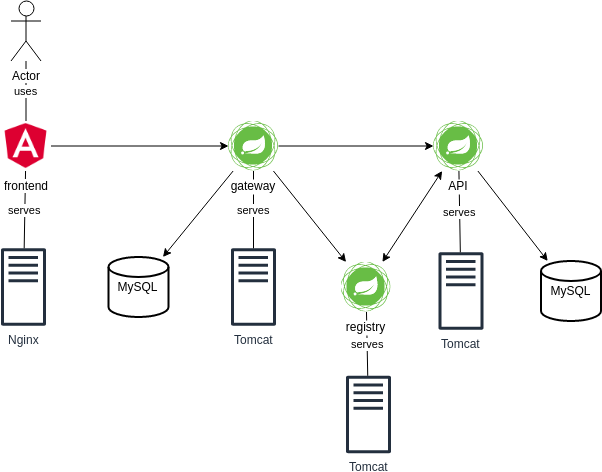
\includegraphics[width=0.7\textwidth]{images/diagrams/gw-archi-detailed.png}
    \caption{Une vue détaillée de l'architecture de l'application Click-and-Run}
    \label{fig:detailed-archi}
\end{figure}

\paragraph{}
La figure \ref{fig:gw-archi} donne un aperçu d'une telle structure.
Voyons avec l'illustration \ref{fig:detailed-archi} sa version détaillée. Je n'y ai inclus que les éléments développés par mes soins et aie omis les éléments externes avec lesquels l'application Click-and-Run interagit.

Détaillons d'abord les noeuds de ce schéma:
\begin{itemize}
    \item \textit{Actor} est l'utilisateur final qui navigue sur nos pages web
    \item Nginx est un \gls{g-server} de fichiers, il sert les fichiers qui lui sont demandés
    \item Tomcat est un serveur applicatif \gls{g-java}, il exécute des applications \gls{g-java} et celles-ci peuvent répondre aux appels qu'on leur fait
    \item \textit{frontend} est l'application Angular qui constitue l'interface que l'utilisateur utilise
    \item \gls{g-mysql} est une base de données
    \item \textit{gateway} est une application \gls{g-spring} qui autorise les demandes et les diriges vers le service demandé
    \item \textit{registry} est une application \gls{g-spring} qui indique où se trouve les services et vérifie leur disponibilité
    \item REST API est une application \gls{g-spring} qui sert des ressources et réponds aux requêtes qu'on lui fait
\end{itemize}
Les flèches indiquent le sens des demandes, le noeud de côté de la queue fait la demande et celui du côté de la pointe répond.
Lorsqu'un verbe est présent sur un lien, le noeud sujet est celui en extrémité du schéma tandis le noeud à l'autre extrémité est le complément d'objet direct.

\paragraph{}
Intéressons nous d'abord à l'application \gls{g-angular}.
Elle est servie par le \gls{g-server} Nginx.
C'est un \gls{g-server} de fichiers, il n'a pas connaissance leur utilité.
C'est le navigateur internet de l'utilisateur qui interprète les instructions du code contenu dans les fichiers.
Tous les fichiers ne sont pas servis en une seule fois, cela ne serait pas idéal.
Seuls les fichiers nécessaires à afficher la page demandée sont données.
Lorsque l'utilisateur navigue dans l'application, cette dernière fera les demandes des fichiers nécessaires à son bon fonctionnement.

\paragraph{}
Peu importe le service que l'application cliente demande, elle doit passée par la passerelle (\textit{gateway} en anglais).

Comme pour chacune des applications \gls{g-java}, un \gls{g-server} Tomcat a la fonction de la faire tourner.
Tomcat est conçu pour exécuter du code \gls{g-java} et écouter les ports réseaux de la machine sur laquelle il est installé pour les diriger vers l'application qu'il sert\cite{noauthor_apache_nodate}.

Celle-ci va tout d'abord s'occuper de vérifier la validité du \gls{a-jwt} transmis avec l'appel (l'authentification est traité en sous-section \ref{subsec:auth-feature}) et ensuite transmettre la demande.
Elle consulte la base de données des utilisateurs pour comparer l'identifiant et le mot de passe lors de l'authentification.
J'ai implémenté un lien direct entre la passerelle et la base de données dans l'application de démonstration mais dans le cas réel de l'infrastructure logicielle d'Altissia, une passerelle existe déjà et elle s'adresse à un service dédié pour quérir les informations des utilisateurs.
Elle a besoin de travailler de pair avec le registre (\textit{registry} en anglais) pour accomplir son travail.

\paragraph{}
Le registre est une application qui tient à jour un carnet d'adresse des différents services.
Elle se base sur le projet Eureka de Netflix\cite{noauthor_aws_2019} pour gérer la découverte des services.
Lorsqu'un service démarre, il renseigne qu'il est prêt à accomplir son devoir au registre.
Le registre va alors contacter fréquemment tous les services ouverts pour s'assurer de leur disponibilité.

En plus de cette tâche, elle configure les services et prend soin de leur évolutivité.
Un service sera donc configuré selon le registre qui est présent sur l'environnement où il est déployé.
L'évolutivité consiste à adapter les ressources allouées au service en fonction de la charge de travail qu'il endure.
C'est aussi elle qui effectue les mesures présentes dans les pages d'administration (voir sous-section \ref{subsec:admin-pages}).

\paragraph{}
L'\gls{a-api} est le composant qui contient la logique métier.
C'est lui qui s'occupe de la validation et le traitement des classeurs Excel.
Il consulte sa base de données lors de la validation et y insère des données lors du traitement.
Selon l'utilisation qui sera fait de Click-and-Run, cette base de données sera remplacée par des appels à des services externes ou une combinaison des deux.
Altissia a fait le choix de structure ses logiciels en microservices où chaque élément a une responsabilité très précise et il ne fait donc pas sens que Click-and-Run gère des ressources métiers en plus de la logique de validation et traitement pour lequel il a été conçu.

Comme on le voit dans la sous-section \ref{subsubsec:dependency-injection}, la différence entre utiliser un service ou une base de données est minime et passer de l'un à l'autre est trivial.

\paragraph{}
L'interface utilisateur et la passerelle sont développées dans le répertoire de code \href{https://github.com/click-and-run/click-and-run-gw}{click-and-run-gw}\fnmark{} tandis que l'\gls{a-api} et le registre le sont dans le répertoire \href{https://github.com/click-and-run/click-and-run}{click-and-run}\fnmark{}.
\fntext{click-and-run-gw: https://github.com/click-and-run/click-and-run-gw}
\fntext{click-and-run: https://github.com/click-and-run/click-and-run}

\subsection{Le serveur avec Spring}
\label{subsec:server-spring}

\paragraph{}
Le \gls{g-server} est implémenté en utilisant le socle d'application \Gls{g-spring} Boot.
C'est une version de \gls{g-spring} où des choix dogmatiques ont été faits sur la manière dont \gls{g-spring} doit être configuré afin de réduire le travail nécessaire à avoir un \gls{g-server} prêt l'emploi.
\Gls{g-spring} est un projet absolument immense et simplifie la vie du développeur dans nombreux contextes.
Je vais me concentrer ici sur quatre aspects:
\begin{itemize}
    \item La base de données
    \item Le réseau
    \item La sécurité
    \item L'injection de dépendance
\end{itemize}

\subsubsection{La base de données}
\label{subsubsec:spring-data-jpa}

\paragraph{}
Son composant \gls{g-spring} Data \acrshort{a-jpa}, qui est bâti par-dessus le projet \gls{g-hibernate}, gère la connexion a la base de données, la représentation des données sous forme d'objet ainsi que la persistance des données.

Ainsi un développeur n'a plus besoin d'écrire la moindre requête \gls{a-sql}.
Il utilise les fonctions fournies par \gls{g-spring} Data \acrshort{a-jpa}.

On peut par exemple voir ci-dessous la classe qui représente le répertoire dans lequel sont stockées les entités des apprenants:
\begin{lstlisting}[language=Java]
@Repository
public interface LearnerRepository extends JpaRepository<Learner,Long> {
    List<Learner> findAllByLoginIn(Collection<String> loginList);
}
\end{lstlisting}
La méthode \lstinline{findAllByLoginIn} n'est pas prévue de base, mais est construire en utilisant les outils fournis par le \gls{g-framework}.

L'appel \lstinline{learnerRepository.save(learners);} utilise une fonction prévue pour sauvegarder plusieurs apprenants en base de données.
À partir de là, \gls{g-spring} Data \acrshort{a-jpa} s'occupe de créer la requête \gls{a-sql} correspondant.

\subsubsection{Le réseau}
\label{subsubsec:spring-web}

\paragraph{}
Le composant \Gls{g-spring} Web est surement le plus utilisé de \gls{g-spring}.
Il permet de transformer les données reçues par le réseau en objet défini par le code \Gls{g-java}.
En cas de tout écart au scénario nominal, il s'occupe de répondre avec le bon code d'erreur à l'appelant.
Il va par exemple répondre "404 \textit{Not Found}" lorsque la ressource recherchée n'existe pas ou encore "500 \textit{Internal Server Error}" lorsque l'application plante et n'est plus capable de formuler une réponse correcte.

\paragraph{}
Voici par exemple une ressource définie par l'\gls{a-api} de Click-and-Run\fnmark{}:
\fntext{J'ai caché certains détails d'implémentation pour simplifier.}
\begin{lstlisting}[language=Java]
@Timed
@PostMapping(value = "/api/registration/validate", produces = MediaType.APPLICATION_JSON_UTF8_VALUE)
public ResponseEntity<Workbook> validateFile(@RequestParam(name = "file") MultipartFile file) {
    log.debug("REST request to /registration/validate with {}", file.getOriginalFilename());

    Workbook workbook = workbookExtendedService.validateWorkbook(file, new RegistrationWorkbook());

    return ResponseEntity.ok(workbook);
}
\end{lstlisting}
Ce code ne contient que très peu de logique et fait surtout appel aux fonctionnalités de \Gls{g-spring} Web. Il indique à quelle URL la ressource doit répondre, avec quel verbe \gls{a-http}, avec quel paramètre et avec quelle réponse.

\subsubsection{La sécurité}
\label{spring-boot-starter-security}

\paragraph{}
Le composant \gls{g-spring} Security s'occupe de fournir des mécanismes de sécurité pour protéger les différentes ressources du serveur avec un degré de granularité personnalisable.
Il vérifie que chaque demande est légitime.

Pour personnaliser ma configuration du \gls{g-server}, j'ai écrit la fonction suivante dans la classe \lstinline{WebSecurityConfigurerAdapter} qui est utilisée par le \gls{g-framework} pour se configurer.
\begin{lstlisting}[language=Java]
@Override
protected void configure(HttpSecurity http) throws Exception {
    http
        .csrf()
        .disable()
        .headers()
        .frameOptions()
        .disable()
    .and()
        .sessionManagement()
        .sessionCreationPolicy(SessionCreationPolicy.STATELESS)
    .and()
        .authorizeRequests()
        .antMatchers("/api/**").authenticated()
        .antMatchers("/management/health").permitAll()
        .antMatchers("/management/**").hasAuthority(AuthoritiesConstants.ADMIN)
        .antMatchers("/swagger-resources/configuration/ui").permitAll()
    .and()
        .apply(securityConfigurerAdapter());
}
\end{lstlisting}
Cet extrait de code désactive des options qui pourrait débouché sur des vulnérabilités si elles n'étaient pas bien utilisées\cite{noauthor_cross-site_nodate},
active un système de cession sans état\fnmark{}, ce qui est possible grâce à l'utilisation d'une authentification par \gls{a-jwt}
\fntext{Sans état signifie que le \gls{g-server} ne doit pas garder les connections de l'utilisateur en mémoire.}
Et enfin, configure les règles d'accès selon l'URL appelée.

Seuls les utilisateurs authentifiés ont accès aux ressources derrière le chemin \lstinline{/api/**}.
Cela concerne par exemple le chemin \lstinline{/api/registration/validate} utilisé dans l'extrait de code de la sous-section \ref{subsubsec:spring-web}.

Les ressources réservées à l'administrateur sont protégées par le chemin \lstinline{/management/**} à l'exception du chemin \lstinline{/management/health} qui indique si le \gls{g-server} est en bonne santé ou non.

\subsubsection{L'injection de dépendance}
\label{subsubsec:dependency-injection}

\paragraph{}
Dans un programme, une partie d'un logiciel dépend très souvent d'autres parties du logiciel.
Si le bout de code considéré devait lui-même récupérer les bouts de code dont il a besoin, il y serait fortement couplé.
C'est-à-dire qu'il doit connaitre le comportement du code dont il dépend sans quoi il ne sait pas s'en servir.
Ce n'est pas forcément une mauvaise, mais dans certains cas, ce n'est pas idéal.

Un exemple classique est la connexion à la base de données.
Établir la connexion à la base de données requiert des informations comme son emplacement, le nom d'utilisateur et le mot de passe.
Si chaque bout de code qui doit accéder à la base de données devait aussi connaitre ces informations, cela donnerait un code assez complexe.

C'est là qu'intervient l'injection de dépendance.
Plutôt que de devoir instancier\fnmark{} sa dépendance, c'est le \gls{g-framework} qui s'en charge et nous le fournit.
\fntext{Créer un exemplaire concret d'une classe ou d'un modèle}
Dans notre cas, c'est \Gls{g-spring} qui s'en charge.

\paragraph{}
Voici deux applications de l'injection de dépendance:
Voici un premier
\begin{lstlisting}[language=Java]
public LoginUnavailableValidator(LearnerRepository learnerRepository) {
    this.learnerRepository = learnerRepository;
}
// TRUNCATED
learnerRepository.findAllByLoginIn(rowsByLogin.keySet()) // TRUNCATED
\end{lstlisting}
Et un deuxième
\begin{lstlisting}[language=Java]
public ExistingUserValidator(UserExtendedResourceApiClient userExtendedResourceApiClient) {
 this.userExtendedResourceApiClient = userExtendedResourceApiClient;
}
// TRUNCATED
Map<String, UserModel> existingEmail = this.userExtendedResourceApiClient.getUserByLoginMapUsingPOST(emails).getBody();
// TRUNCATED
\end{lstlisting}
Le premier extrait de code fait appel à une base de données tandis que le deuxième appelle un \gls{a-api} en passant par le réseau.
Le développeur ne voit pas la différence, car c'est \Gls{g-spring} qui s'est chargé de fournir les dépendances nécessaires.

En l'occurrence, il peut être intéressant de noter que la méthode du deuxième extrait de code est générée par un outil appelé Swagger sur base du code de la ressource.
Je parle bien d'une ressource telle que celle montrée en exemple dans la sous-section \ref{subsubsec:spring-web}.
Une autre différence est que le premier extrait de code vient de Click-and-Run tandis que le second est un extrait d'un service d'Altissia tournant actuellement en production.
La transition entre les deux est donc triviale.

\paragraph{}
Ce mécanisme est très utile pour implémenter le patron de conception de la stratégie, comme vu dans la sous-section \ref{subsec:class-diagram}.


\subsection{L'interface cliente avec Angular}
\label{subsec:frontend-angular}
TODO
